
%----------------------------------------------------------------------------
\chapter{Használati útmutató}
%----------------------------------------------------------------------------

Ez a fejezet tartalmazza az alkalmazás jelenlegi formájának a telepítési instrukcióit, továbbá bemutatja a fentebb részletezett funkciókat működés közben. Jelenleg az alkalmazás még nem konténerízalt formátumú így szükségünk lesz segédeszközökre. 
%----------------------------------------------------------------------------
\section{Telepítés}
%----------------------------------------------------------------------------

Használat előtt győződjünk meg, hogy rendelkezünk az alábbiakkal:
\begin{itemize}
	\item java 11
	\item UPAAL elérés regisztrálva van a környezeti változókba
	\item API tesztelő alkalmazás pl: Postman\footnote{Postman letölthető: \url{https://www.postman.com/}}
	\item Egy Java fejlesztői eszköz pl: InteliJ IDEA\footnote{IDEA letölthető: \url{https://www.jetbrains.com/idea/download}}
\end{itemize}

A szoftver komponensek közül a Webszervert kell megnyitni az IDEA segítségével. Az OpenProject funkciót használva tallózzuk ki a webszerver gyökér mappájában levő \textit{pom.xml}-t.  Miután látható a projekt a fejlesztői környezetbe, keressük ki a \textit{configuration.properties} fájlt, ami tipikusan az \textit{/src/main/resource mappában} lesz elhelyezve, és állítsuk be az alábbiakat:

\begin{lstlisting}[language=]
headless.gamma.path=<A Headless Gamma teljes elérése>
headless.generator.path=<A Headless Generator teljes elérése>
root.of.workspaces.path=<Annak a mappának a teljes elérése, ami a munaktereket fogja tartalmazni>
\end{lstlisting}

Fontos, hogy a két headless eclipse elérése tartalmazza az eclipse kulcsszót az elérés végén, mivel ez lesz a .exe állomány (pl: C:/opt/gammaapi/eclipse). A két headless eclipse-t exportálással tudjuk előállítani, viszont a Webszerver komponens tartalmazni fogja ezeket, ennek ellenére a konfigurációt el kell végezni.
Innentől kezdve az IDEA-ból elindítható az alkalmazás és a \textit{localhost:8080}-on fog figyelni a kérésekre. Az alábbiakban részletezni fogom, hogyan tudjuk tesztelni az alkalmazást.
%----------------------------------------------------------------------------
\section{Tesztelés}
%----------------------------------------------------------------------------

Tesztelés során a gamma teszt projektet\footnote{https://github.com/ftsrg/gamma/tree/master/tests} fogom használni, mivel tartalmaz komplex gamma művelethalmazokat. Minden kérést a Postman segítségével fogok összeállítani és elküldeni, majd megtekintjük a szerveren milyen hatása volt.

\paragraph{Workspace létrehozás} Mivel jelenleg a szerverünk nem tárol semmit ezért hozzunk létre három munkateret. A kiadott HTTP kérések ugyanazok lesznek hiszen nem utazik semmi a paraméterekben ezt \aref{fig:addworkspace_test} ábrán lehet megtekinteni.
\begin{figure}[!ht]
	\centering
	
\includegraphics[keepaspectratio]{figures/addworkspace_test.PNG}
	\caption{Munkatér regisztráció HTTP kérés}
	\label{fig:addworkspace_test}
\end{figure}

\noindent A válasz üzenet tartalmazni fogja egyesével a  munkatér azonosítókat:
\begin{lstlisting}[language=]
567e54cd-289d-48c6-84fb-2d971f8ff9de
99b21cd3-6778-47db-9e00-29e3ce2420be
394d3fc8-5abb-4f40-a13d-252185d8c9bf
\end{lstlisting}

Ezt a mappa kezelő segítségével is ellenőrizni tudjuk, ahogy \aref{fig:workspace_infile} ábrán látható is. Az alkalmazáshoz tartozik egy  konfigurációs fájl, amiben megadható, hogy a workspace-k hova jöjjenek létre.

\begin{figure}[!ht]
	
\includegraphics[width=\textwidth, keepaspectratio]{figures/workspace_infile.PNG}
	\caption{Munkaterek tárolása}
	\label{fig:workspace_infile}
\end{figure}

\paragraph{Projekt importálás} A gamma teszt projektet fogjuk importálni két különböző munkatérbe. Nagyon fontos, hogy a projekt tartalma archiválva legyen és az archivált fájl neve megegyezzen a projekt nevével. A kérésben ebben az esetben meg kell adjuk a munkatér azonosítót az URL-ben és a kérés törzsébe fel kell vennünk az említett archivált állományt és a projekt tulajdonos e-mail címét. A példánkra illeszkedő kérést \aref{fig:add_project_request} ábra mutatja be.


\begin{figure}[!ht]
	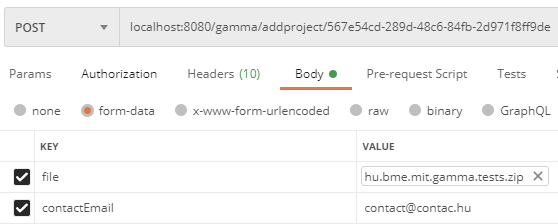
\includegraphics[keepaspectratio]{figures/add_project_request.PNG}
	\caption{Projekt importálás kérés}
	\label{fig:add_project_request}
\end{figure}

Ezen kérések hatására létrejönnek a projektek a megfelelő munkaterek alá, ezt \aref{fig:add_project_result} ábrán is meglehet tekinteni.

\begin{figure}[!ht]
	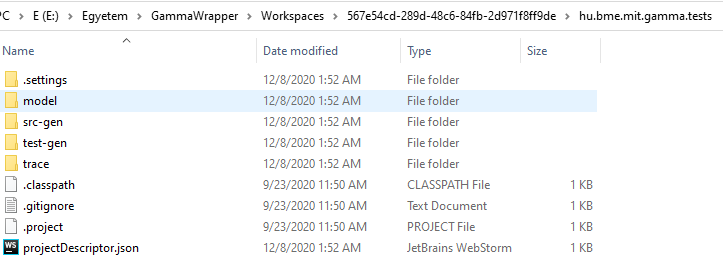
\includegraphics[width=150mm, keepaspectratio]{figures/add_project_result.PNG}
	\caption{Projekt importálás eredmény}
	\label{fig:add_project_result}
\end{figure}

\paragraph{Gamma műveletek futtatása} Tekintsük át a teszt projektben szereplő /model/SSM/System/Mission.ggen fájlt.

\begin{lstlisting}[language=]
import "Mission.gcd"
import "GroundStation/GroundStation.gcd"
import "Spacecraft/Spacecraft.gcd"

code {
	component : GroundStation
	language : java
}

code {
	component : Spacecraft
	language : java
}

code {
	component : Mission
	language : java
}

analysis {
	component : Mission
	language : UPPAAL
	transition-coverage
	constraint : {
		minimum-orchestrating-period : 999 ms
		maximum-orchestrating-period : 999 ms
	}
}

verification {
	language : UPPAAL
	file : "Mission.xml"
	query-file : "Mission.q"
	optimize : true
	test-language : java
}
\end{lstlisting}
Látható, hogy három kódgenerálást és egy verifikációt is fogunk végezni a felső három sorban importált modelleken. Futtassuk ezt az állományt a két projektünkön , \aref{fig:request_gamma_operation} kérés alapján, annyi különbséggel, hogy a megfelelő munkatér azonosítót adjuk meg. Az URL-ben utazik a munkatér azonosító, projektnév és a .ggen fájl elérése a projekten belül.
\begin{figure}[!ht]
	
\includegraphics[width=150mm, keepaspectratio]{figures/request_gamma_operation.PNG}
	\caption{Gamma műveletek futtatására kérés}
	\label{fig:request_gamma_operation}
\end{figure}

Ennek hatására a hoszt szerveren elindul a két folyamat, erről a \texttt{tasklist | findstr eclipse} parancs segítségével győződhetünk meg:
\begin{lstlisting}[language=]
eclipse.exe				1008 Console			2  1,012,184 K
eclipse.exe				1272 Console			2  	 863,800 K
\end{lstlisting}

A projektek jelenleg feldolgozás alatt állnak, így semmilyen műveletet nem lehet rajtuk végezni. Ha mégis küldünk egy kérést erre a projektre, akkor az alábbi hibaüzenet fogjuk kapni a szervertől:

\begin{lstlisting}[language=]
{
	"code": 503,
	"message": "There is an in progress operation on this project, try again later!"
}
\end{lstlisting}

\paragraph{Gamma műveletek leállítása} Előfordulhat, hogy valamiért egy művelet túl sok ideig fut, ezzel zárolva a teljes projektet, ezt fel lehet oldani \aref{fig:stop_gamma_request} ábrán levő kérés segítségével. A kérésben URL-jében a projektet meghatározó munkatér-projektnév páros kell utazzon, a törzs üres maradhat. Jelenlegi esetben nem merül fel ilyen hiba, mivel mindkét folyamat kb 5-7 perc alatt lefut, viszont a tesztelés céljából leállítjuk az egyiket.


\begin{figure}[!ht]
	
\includegraphics[width=150mm, keepaspectratio]{figures/stop_gamma_request.PNG}
	\caption{Futó headless gamma leállítása}
	\label{fig:stop_gamma_request}
\end{figure}

Eredményként annyit tapasztalunk, hogy megint használhatóvá válik a projekt.

\paragraph{Gamma eredmények lekérése} Végezetül szükségünk van a generált eredmény állományokra. Ezt \aref{fig:get_result_request} ábrán levő kéréssel tudjuk megvalósítani, az URL-ben a megszokott munkatér-projektnév páros utazik, a törzsben pedig egy olyan json objektum van, amiben listaként szerepelnek az egyes állományok relatív elérése. A Postman-be ilyenkor nem csak el kell küldeni a kérést hanem a \textit{Send and Download} gombra kell kattintani, így tudni fogja, hogy fájlt fog kapni a szervertől.

\begin{figure}[!ht]
	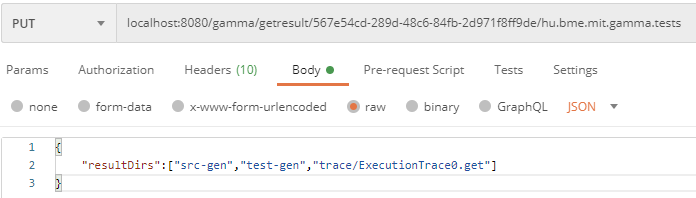
\includegraphics[width=150mm, keepaspectratio]{figures/get_result_request.PNG}
	\caption{Eredmény lekérés}
	\label{fig:get_result_request}
\end{figure}

Eredményül pedig a megadott állományokat kapjuk becsomagolva, \aref{fig:result_zip} ábrán a \textit{src-gen} tartalma látható. 

\begin{figure}[!ht]
	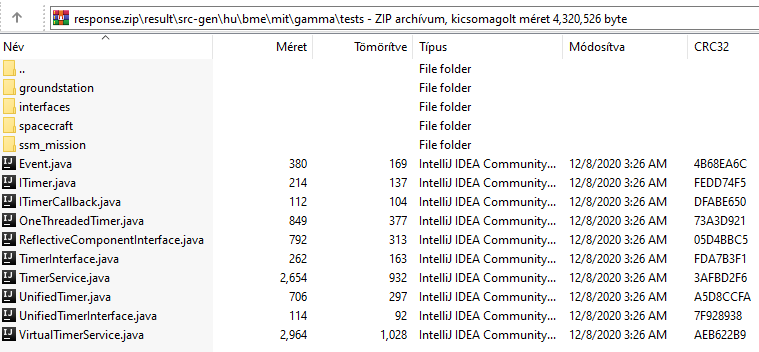
\includegraphics[width=150mm, keepaspectratio]{figures/result_zip.PNG}
	\caption{Eredmény fájl tartalma}
	\label{fig:result_zip}
\end{figure}
\paragraph{További funkciók} Lehetőségünk van projekt törlésre is, erre \aref{fig:delete_project_request} ábrán látható kérés szolgál. Az URL-ben utazó munkatér és projektnév párossal azonosított projekt teljes tartalma törlésre kerül.


\begin{figure}[!ht]
	
\includegraphics[width=\textwidth, keepaspectratio]{figures/delete_project_request.PNG}
	\caption{Projekt törlés kérés}
	\label{fig:delete_project_request}
\end{figure}

A lejáró projektet dátumát egy naponta futó időzítő figyeli, ha talál olyan projektet, aminek a lejárati dátuma a mai nap, akkor azt törli. \Aref{fig:extend_expiration_req} ábrán levő kéréssel tudjuk 30 nappal meghosszabbítani a lejárati dátumot.

\begin{figure}[!ht]
	
\includegraphics[width=\textwidth, keepaspectratio]{figures/extend_expiration_req.PNG}
	\caption{Projekt lejárati dátum meghosszabbításra szolgáló kérés}
	\label{fig:extend_expiration_req}
\end{figure}